\documentclass[twoside]{article}

\usepackage{aistats2020}
% If your paper is accepted, change the options for the package
% aistats2020 as follows:
%
% \usepackage[accepted]{aistats2020}
%
% This option will print headings for the title of your paper and
% headings for the authors names, plus a copyright note at the end of
% the first column of the first page.

% If you set papersize explicitly, activate the following three lines:
%\special{papersize = 8.5in, 11in}
%\setlength{\pdfpageheight}{11in}
%\setlength{\pdfpagewidth}{8.5in}

% If you use natbib package, activate the following three lines:
%\usepackage[round]{natbib}
%\renewcommand{\bibname}{References}
%\renewcommand{\bibsection}{\subsubsection*{\bibname}}

% If you use BibTeX in apalike style, activate the following line:
%\bibliographystyle{apalike}

\usepackage{natbib}
\usepackage{amsfonts}       % blackboard math symbols
\usepackage{amsmath}
\usepackage{graphics}
\usepackage{graphicx}
\usepackage{caption}
\usepackage{subcaption}

\graphicspath{{../diagrams/}}

% math definition

\newcommand{\yM}{\mathbf{Y}}
\newcommand{\yV}{\mathbf{y}}
\newcommand{\fM}{\mathbf{F}}
\newcommand{\fV}{\mathbf{f}}
\newcommand{\xM}{\mathbf{X}}
\newcommand{\xV}{\mathbf{x}}
\newcommand{\K}{\mathbf{K}}
\renewcommand{\L}{\mathbf{L}}
\newcommand{\R}{\mathbb{R}}
\newcommand{\uM}{\mathbf{U}}
\newcommand{\uV}{\mathbf{u}}
\newcommand{\zM}{\mathbf{Z}}
\newcommand{\zV}{\mathbf{z}}
\newcommand{\bound}{\mathcal{L}}
\newcommand{\I}{\mathbf{I}}
\newcommand{\lambdaM}{\mathbf{\Lambda}}
\newcommand{\aM}{\mathbf{A}}
\newcommand{\hV}{\mathbf{h}}
\newcommand{\bV}{\mathbf{b}}
\newcommand{\wM}{\mathbf{W}}
\newcommand{\wV}{\mathbf{w}}
\newcommand{\phiM}{\mathbf{\Phi}}
\newcommand{\phiV}{\mathbf{\phi}}
\newcommand{\KL}[2]{\text{KL}\left( #1\,\|\,#2 \right)}
\newcommand{\expectationDist}[2]{\left\langle #1 \right\rangle _{#2}}
\newcommand{\diff}{\text{d}}
\newcommand{\J}{\mathbf{J}}
\newcommand{\gaussianDist}[3]{\mathcal{N}\left(#1|#2,#3\right)}
\newcommand{\tr}[1]{\text{tr}\left(#1\right)}

\newcommand{\ie}{\textit{i.e.}}

\usepackage{xspace}
\newcommand{\acr}[1]{\textsc{#1}\xspace}
\newcommand{\us}{\acr{NFW}}
\newcommand{\sivi}{\acr{SIVI}}


\begin{document}

% If your paper is accepted and the title of your paper is very long,
% the style will print as headings an error message. Use the following
% command to supply a shorter title of your paper so that it can be
% used as headings.
%
%\runningtitle{I use this title instead because the last one was very long}

% If your paper is accepted and the number of authors is large, the
% style will print as headings an error message. Use the following
% command to supply a shorter version of the authors names so that
% they can be used as headings (for example, use only the surnames)
%
%\runningauthor{Surname 1, Surname 2, Surname 3, ...., Surname n}

\twocolumn[

\aistatstitle{Variational Inference with Non-invertible Flows}

\aistatsauthor{ Author 1 \And Author 2 \And  Author 3 }

\aistatsaddress{ Institution 1 \And  Institution 2 \And Institution 3 } ]

\begin{abstract}
We explore the possibility of extending normalizing flows with non-invertible transformations for variational inference. We show that the probability density function of the resulting distribution can be derived analytically, but it depends on all the real roots of the transformation equation.  To address this limitation, we develop non-invertible flows (NFW), a variational inference method with non-invertible transformations by approximating the degenerate conditional distribution of transformation with a normal distribution with a small variance. This brings a close connection to semi-implicit variational inference (SIVI) methods. Unlike SIVI methods, our variational lower bound does not require a large sample size and does not need to run a Markov Chain Monte Carlo method during variational inference. We demonstrate NFW on several tasks, including variational autoencoders, image imputation and Bayesian neural network regression, and show that it can capture complex distributions and deliver state-of-the-art performance on various tasks.
\end{abstract}

\section{Introduction}

Variational inference (VI) is an important family of methods for scaling probabilistic modeling for real world problems. VI converts the intractable posterior estimation of Bayesian inference into an optimization problem, in which the task is to search for the parameters of a chosen distribution that minimizes the Kullback-Leibler (KL) divergence between the parametric distribution and the true posterior distribution. The objective function of optimization is often formulated as optimizing a variational lower bound of the log marginal likelihood, which is also called the evidence lower bound (ELBO). Two major challenges of VI are 1) calculation of the integral in the ELBO and 2) expressiveness of variational distributions. 
%Classical VI methods relies on a closed form estimation of the KL divergence, which heavily re
A popular approach to address the problem of the integral calculation is to approximate the ELBO with Monte Carlo samples. By using reparameterizable distributions, a lower variance estimation is achievable with a relatively small number of samples. This requires a rich family of reparameterizable variational distributions. Many works focus on developing reparameterizable representations of known distributions \citep{RuizEtAl2016,NaessethEtAl2016,FigurnovEtAl2018}. This significantly extends the choices of variational distributions, but for large scale probabilistic models, a good variational distribution often needs to be  high dimensional, highly correlated among dimensions, and cannot be constructed with known distribution families. 

Normalizing flows (NF), proposed by \cite{JimenezRezendeMohamed2015}, constructs complex probability distributions via transforming random variables from a simple probability distribution with a known probability density function (PDF). By restricting the transformation to be invertible, a resulting distribution can be used for variational inference, because 1) it is reparameterizable, as a sample can be formulated as a function of the parameters of transformation, 2) the PDF can be calculated in closed form. The main limitation of NF is the computational expensive PDF calculation, in which the log determinant of the Jacobian of the transformation needs to be computed. This is impractical for distributions with thousands of dimensions, e.g., the posterior of a  Bayesian neural network (BNN). Many follow-up works \citep{KingmaEtAl2016, DinhEtAl2017, HuangEtAl2018} address this problem by a careful construction of the transformation such that the Jacobian is a triangular matrix. This allows efficient computation of the log determinant of the Jacobian, but is at the cost of enforcing an order of dependency among dimensions and being slow at generating samples, since the samples have to go through an autoregressive model.

In this paper, we explore the possibility of extending NF with non-invertible transformations. The major challenge of using non-invertible transformations is to calculate the PDF of the resulting distribution. The change of variable formula used to derive the PDF of NF is no longer applicable. We show that, if the dimensionality of the initial distribution is greater than or equal to the dimensionality of the resulting distribution, the PDF can be derived analytically, but is not practical because it depends on all the real roots of the transformation equation. To address this limitation, we approximate the conditional distribution of the transformation, which is a Dirac delta distribution, with a normal distribution with a small variance. With the approximated conditional distribution, we develop non-invertible flows (\us),  a variational inference method using a non-invertible transformation, in which a variational lower bound is derived by introducing an auxiliary distribution. The formulation of connecting a simple random variable to the target variable with a non-invertible function in variational posterior is closely related to semi-implicit variational inference (SIVI) methods \citep{YinZhou2018, TitsiasRuiz2019, MolchanovEtAl2019}. Unlike the SIVI methods, our variational lower bound works well with a small number of samples and does not need to run a Markov Chain Monte Carlo method during variational inference. We show that the auxiliary distribution in \us produces a similar regularization effect as the log determinant in NF, which demonstrates a strong connection between the NF-based methods and the SIVI methods. 

\section{Variational inference with implicit distribution}

Consider a set of observed variables $\yV$ and a set of latent variables $\xV$, for which a probabilistic model is defined in terms of a conditional distribution over the observed variables $p(\yV|\xV)$ and a prior distribution over the latent ones $p(\xV)$. VI is often applied to estimate the intractable posterior distribution $p(\xV|\yV)=\int p(\yV|\xV)p(\xV)/p(\yV)\diff \xV$. VI solves this intractable posterior estimation by converting the integral calculation into an optimization problem, where we define a parametric distribution as the variational posterior and optimize the parameters of the variational posterior to match the true posterior distribution. This optimization is often formulated as minimizing the KL divergence between the variational posterior and the true posterior,
\begin{equation}
\begin{split}
&\KL{q_\theta(\xV)}{ p(\xV|\yV)} = \\
& \expectationDist{\log p(\yV, \xV)-\log q_\theta(\xV)}{q_\theta(\xV)} - \log p(\yV),
\end{split}
\end{equation}
where $q_\theta(\xV)$ is the variational posterior and $\theta$ are the parameters of the variational posterior. Note that the marginal likelihood term $\log p(\yV)$ is independent of $q_\theta(\xV)$. VI focuses on minimizing the first term $\expectationDist{\log p(\yV, \xV)-\log q_\theta(\xV)}{q_\theta(\xV)}$, which is often referred to as variational lower bound or ELBO.

%\begin{equation}
%\theta^* = \arg \max_\theta \bound_\theta
%\end{equation}

Despite the fact that the form of the variational posterior is chosen by hand, for most sophisticated probabilistic models it is hard to find a variational posterior distribution that gives a closed-form variational lower bound. Instead of simplifying the model and variational posterior for a closed form variational lower bound, stochastic variational inference (SVI) optimizes the variational posterior with respect to a Monte Carlo estimate of the variational lower bound,
\begin{equation}
\bound \approx \frac{1}{K} \sum_{i=1}^K \log p(\yV, \xV_i)-\log q_\theta(\xV_i), \quad \xV_i \sim q_\theta(\xV). \label{eqn:elbo}
\end{equation}
This allows us to use more sophisticated probabilistic models and variational posteriors. The variational posterior is typically optimized via gradient optimization. To directly estimate the gradient of a variational posterior from (\ref{eqn:elbo}), the variational posterior needs to 1) have a closed form PDF, 2) be reparameterizable.
%
Note that in (\ref{eqn:elbo}), to estimate the gradient of the variational parameters with respect to the variational lower bound, the gradient not only needs to be estimated from the log PDF $\log q(\xV)$ but also needs to chain through the individual samples, \ie, 
\begin{equation}
\frac{\partial \bound}{\partial \theta} = -\frac{\partial \log q(\xV_i)}{\partial \theta} + \sum_{i=1}^K \frac{\partial \bound}{\partial \xV_i} \frac{\partial \xV_i}{\partial \theta}. 
\end{equation}
%
This requires the random variable to be defined as a transformation of a standard probability density. For example, a normally distributed variable can be written as $x = \mu + \sigma\epsilon$, where $\mu$ and $\sigma^2$ are the mean and variance of the normal distribution and $\epsilon$ follows a normal distribution with zero mean and unit variance $\epsilon \sim \mathcal{N}(0, 1)$. This is known as  the explicit reparameterization \citep{KingmaWelling2014}. 

%Another example of such transformation, a scalar random variable can be formulated as the uniform distributed variable transformed by its inverse cumulative distribution function (CDF), \ie, $x = F^{-1}(\epsilon)$, where $\epsilon \sim \mathcal{U}[0, 1]$ and $F(x)$ is the CDF \citep{FigurnovEtAl2018}.

\subsection{Change of Variable}

The reparameterization trick allows us to build low variance estimators for a subset of known probabilistic distribution for SVI, among which the scalar normal distribution remains the most practical choice. This enables wide usage of mean field approximations in SVI, $q(\xV) = \prod_{k=1}^N q(x_k)$. However, mean field is a poor assumption for the random variables that are strongly correlated in the posterior. 

Normalizing flows, introduced by \cite{JimenezRezendeMohamed2015}, provide a powerful approach to generate a complex probability distribution by applying the change of variable formula. It starts with an initial random variable $\zV_0 \in \R^D$ and applies the transformation functions $f_1, \ldots, f_T$, 
$$
\zV_0 \sim q(\zV_0), \quad  \zV_t = f_t(\zV_{t-1}),\quad \forall t=1,\ldots, T.
$$
The PDF of $\zV_0$ is denoted as $q(\zV_0)=g(\zV_0)$. Drawing a sample from the resulting distribution $q(\zV_T)$ is straight-forward, which can be done by drawing a sample from the initial distribution and applying the series of transformation functions.
%
All the transformation functions need to be invertible. According the change of variable formula, the PDF of the target variable can be formulated as
\begin{equation}
q(\zV_T) = g(f_1^{-1} \circ \ldots \circ f_T^{-1}(\zV_T)) \prod_{t=1}^T \left| \frac{\partial f_t^{-1}(\zV_t)}{\partial \zV_t}\right|. \label{eqn:nf_pdf}
\end{equation}
%
Sampling from the resulting distribution and evaluating the original PDF can both be done efficiently. However, the computation of the Jacobian of the inverse transformation can be expensive when the dimensionality of the probability distribution gets high. \cite{KingmaEtAl2016}  propose inverse autoregressive flows (IAF) to tackle the computational challenge of the above determinant by constructing the transformation function of which the Jacobian is an triangular matrix. This reduces the complexity of the calculation from $O(D^2)$ to $O(D)$. Such a transformation is restrictive, as only an output dimension of the transformation can depend on previous dimensions but not the other way around. The computation suffers from the common limitations of autoregressive networks: slow evaluation and the need of additional tricks for gradient computation.

\subsection{Non-invertible Transformation}

An obvious extension to NF is to consider non-invertible transformations. However, the challenge is that the PDF formula (\ref{eqn:nf_pdf}) is no longer applicable. \textit{What is the PDF of the target random variable after a non-invertible transformation?}

We start off by looking into how the PDF is derived for 1D cases. Following the rule of marginalization, the PDF of the target variable $x$ that is transformed from an initial random variable $z$ with the function $f$ is defined as 
\begin{equation}
\begin{split}
q(x) = \int q(x|z) q(z) \diff z &= \int \delta\left(x - f(z)\right) g(z) \diff z\\
 &= g(f^{-1}(x)) \left|\frac{\partial f^{-1}(x)}{\partial x}\right|,
\end{split}
\label{eqn:dirac_invertible}
\end{equation}
where the PDF of $z$ is $g(z)$ and $x$ has a deterministic relation with $z$: $x=f(z)$. In this case, the conditional distribution $q(x|z)$ is degenerate, which can be represented by a Dirac delta function. The resulting degenerate PDF returns an infinite density at the location $f(z)$ and zero everywhere else, \ie, $q(x|z) = \delta\left(x - f(z)\right)$. If $f$ is invertible, using the properties of Dirac delta function \citep{Arfken1985}, the PDF $q(x)$ can be derived in closed form as shown in (\ref{eqn:dirac_invertible}), which leads to (\ref{eqn:nf_pdf}).

If $f$ is non-invertible, the PDF can also be derived in closed form,
\begin{equation}
\begin{split}
q(x)  &= \int \sum_{i, f(z_i)=x, f'(z_i)\neq0} \frac{\delta(z - z_i)}{|f'(z_i)|} g(z) \diff z\\
 &= \sum_{i, f(z_i)=x, f'(z_i)\neq0} \frac{g(z_i)}{|f'(z_i)|}, \label{eqn:pdf_noninvertible}
\end{split}
\end{equation}
where $\{z_i\}$ are all the real roots of the equation $x=f(z)$. Fig.\,\ref{fig:nfw_1d_example} shows an example of transforming a standard normal distribution $z \sim \mathcal{N}(0,1)$ with a  quadratic function $x=z^2+4$. Following (\ref{eqn:pdf_noninvertible}), the PDF of the resulting distribution is, 
\begin{equation*}
q(x) =   
\begin{cases}
  0 & \quad x<4, \\
\frac{q(z=-\sqrt{x-4})}{|f'(-\sqrt{x-4})|}+\frac{q(z=\sqrt{x-4})}{|f'(\sqrt{x-4})|}  & \quad x>4.
\end{cases}
\end{equation*}
As shown in the example, the PDF is zero when no real roots exist and the PDF is a sum of multiple terms, one for each real root, in which each term takes the same form as the PDF under an invertible transformation in (\ref{eqn:dirac_invertible}).

\begin{figure*}
     \begin{subfigure}[t]{0.45\textwidth}
         \centering
         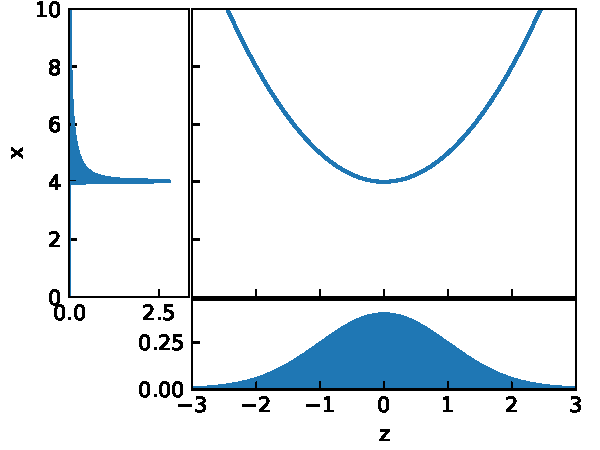
\includegraphics[width=0.9\textwidth]{non-invertible_1d.pdf} 
         \caption{}
         \label{fig:nfw_1d_example}
     \end{subfigure}
     \begin{subfigure}[t]{0.45\textwidth}
         \centering
         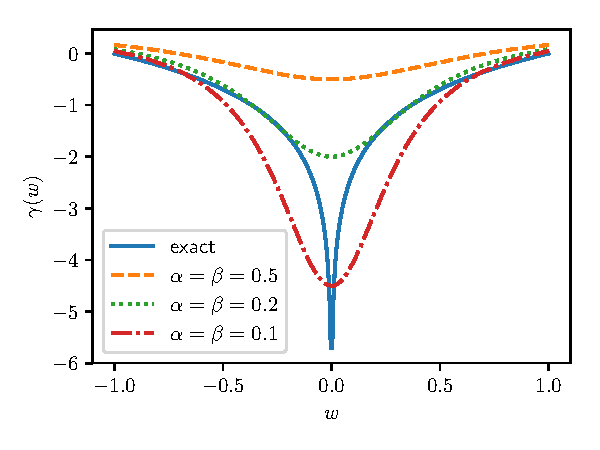
\includegraphics[width=0.95\textwidth]{regulerizer.pdf} 
         \caption{}
         \label{fig:regularization}
     \end{subfigure}
\caption{(a) An example of a univariate distribution under a non-invertible transformation. The x-axis shows the initial distribution $z \sim \mathcal{N}(0, 1)$ and the transformation is a quadratic function $x=z^2+4$. The resulting distribution is visualized along the y-axis. (b) The comparison of the "regularization" term in the exact PDF and our variational approximation under a linear transformation $x=wz$. The x-axis shows $w$ and the y-axis shows the value of the regularization term.  The solid curve indicates the exact PDF and the other curves indicates our variational approximation with different $\alpha$ and $\beta$.} 
\end{figure*}

For multivariate distributions, a similar result can also be obtained. When the dimensionality of the initial variable $D_z$ is larger than the dimensionality of the target variable $D_x$, using the co-area formula from geometric measure theory \citep{Federer1969}, a similar formula can be derived for multivariate distributions,
\begin{equation}
q(\xV)  = \int \delta\left(\xV - f(\zV)\right) g(\zV) \diff \zV=  \int_{f^{-1}(\xV)}  \frac{g(\zV)}{\left|\J_z^\top\J_z\right|^{\frac{1}{2}}}  \diff \zV,
\end{equation}
where $\J_z$ is the Jacobian of the function $f$ at $\zV$ and the integral is over $f^{-1}(\xV)$, the surface defined by $f(\zV) = \xV$. Note that, the denominator in the multidimensional formula is different from the one in the univariate case, due to the fact that the Jacobian of a multivariate transformation may not be a square matrix. If $x$ is a scalar, the PDF becomes a special case,
\begin{equation}
q(x)  =  \int_{f^{-1}(x)}  \frac{g(\zV)}{\left|\nabla f\right|}  \diff \zV,
\end{equation}
where the denominator is the norm of the gradient of the function $f$. If the dimensionality of the initial variable $D_z$ is smaller than the dimensionality of the resulting variable $D_x$, the PDF is no longer finite, as it is a degenerate distribution.



\section{Variational Non-invertible Flows}

Although the PDF of a random variable generated from a non-invertible transformation can be formulated analytically, it depends on all the real roots of the transformation equation, which is non-trivial for complex transformation functions, as the conditional distribution $q(\xV|\zV)$ is degenerate. To calculate the PDF at a given $\xV$, we are required to find the corresponding values of $\zV$ that map to $\xV$, which is formulated as the roots of the transformation equation. To avoid the root finding, we approximate the degenerate conditional distribution $q(\xV|\zV)$ with a normal distribution with a small variance, which can be viewed as an approximation to the Dirac delta distribution. The Dirac delta function can be defined as the limit of the Gaussian PDF as the variance approaches zero, \ie, $\delta(\xV) = \lim_{\alpha \rightarrow 0} \gaussianDist{\xV}{0}{\alpha\I}$. We avoid the infinite probability density problem by setting $\alpha$ to be a small positive number, i.e.,
\begin{equation}
\begin{split}
q(\xV|\zV) = \delta(\xV - f(\zV)) &= \lim_{\alpha \rightarrow 0} \gaussianDist{\xV}{f(\zV)}{\alpha\I}\\
 &\approx \gaussianDist{\xV}{f(\zV)}{\alpha\I}.
\end{split}
\end{equation}
As a result, $q(\xV|\zV)$ gives a small probability mass around $\xV$, which avoids $p(\xV)$ becoming degenerate if $D_x > D_z$. We no longer have an analytical expression for $q(\xV)$, which needs to be estimated from the intractable marginal distribution $q(x) = \int q(x|z) q(z) \diff z$.

\subsection{Variational lower bound with auxiliary distribution}

As $q(\xV)$ is no longer in closed form, we cannot directly use it as a variational posterior for VI. To avoid this problem, we introduce an auxiliary distribution $\tilde{q}(\zV|\xV)$. In this paper, we use a normal distribution $\tilde{q}(\zV|\xV)= \gaussianDist{\zV}{\tilde{f}(\xV)}{\beta\I}$, where $\tilde{f}$ is a function parameterized as a deep neural network (DNN), but other distributions are also applicable. With the auxiliary distribution, we define an unbiased estimator of the marginal likelihood $p(\yV)$ by drawing Monte Carlo samples,
\begin{equation}
\begin{split}
p(\yV) &= \int q(\xV, \zV) \frac{p(\yV, \xV) \tilde{q}(\zV | \xV)}{q(\xV, \zV)} \diff \xV \diff \zV \\
&\approx \frac{1}{N} \sum_{i=1}^N \frac{p(\yV, \xV_i) \tilde{q}(\zV_i | \xV_i)}{q(\xV_i, \zV_i)}, \quad \xV_i, \zV_i \sim q(\xV, \zV), \label{eqn:importance_sampling}
\end{split}
\end{equation}
where $N$ is the number of drawn samples and $q(\xV, \zV) = q(\xV|\zV) q(\zV)$. Using Jensen's inequality, a variational lower bound can be derived for the log marginal likelihood,
\begin{equation}
\begin{split}
\log p(\yV) &= \log \int q(\xV, \zV) \frac{p(\yV, \xV) \tilde{q}(\zV | \xV)}{q(\xV, \zV)} \diff \xV \diff \zV \\
&\geq  \int q(\xV, \zV) \log \frac{p(\yV, \xV) \tilde{q}(\zV | \xV)}{q(\xV, \zV)} \diff \xV \diff \zV = \bound. \label{eqn:nfw_bound}
\end{split}
\end{equation}
We denote the above lower bound as $\bound$. Note that, although we have an extra term in the nominator, it is still a lower bound of the log marginal likelihood. The relation to the usual variational lower bound can be seen by re-arranging the bound as follows:
\begin{equation}
\bound = \int q(\xV) \log \frac{p(\yV, \xV) }{q(\xV)} \diff \xV \diff \zV - \expectationDist{\KL{\tilde{q}(\zV|\xV)}{q(\zV|\xV)}}{q(\xV)},
\end{equation}
where $q(\xV) = \int q(\xV| \zV) q(\zV) \diff \zV$ is the marginal variational posterior and $q(\zV|\xV)$ is the true "posterior" of the variational distribution $q(\xV, \zV)$. The first term is the usual variational lower bound. As the KL divergence is greater than or equal to zero, $\bound$ is a lower bound of the first term and they become equal only if the auxiliary distribution $\tilde{q}(\zV|\xV)$ is the same as the true variational posterior distribution $q(\zV|\xV)$ for all $\xV$.


\subsection{Connection to normalizing flows}

We approximate  the lower bound of \us  with Monte Carlo samples,
\begin{equation}
\bound \approx \frac{1}{K} \sum_{i=1}^K\left( \log \frac{p(\yV, \xV_i) }{q(\zV_i)}+  \log \frac{\tilde{q}(\zV_i | \xV_i)}{q(\xV_i|\zV_i)}  \right) , \quad \zV_i \sim q(\zV), \label{eqn:mc_bound}
\end{equation}
where $\xV_i = f(\zV_i) + \alpha^{\frac{1}{2}} \epsilon_i$, $\epsilon_i \sim \mathcal{N}(0, \I)$. Note the first term is the same as the one for NF, which is 
\begin{equation}
\bound \approx \frac{1}{K} \sum_{i=1}^K   \left(\log \frac{p(\yV, \xV_i)|_{\xV_i = f(\zV_i)} }{q(\zV_i)}+  \log \left| \J_{\zV_i} \right| \right). \label{eqn:mc_bound_nf}
\end{equation}
The first term gives a large value in the location where the likelihood is high. Optimizing with respect to this term alone will lead to the variational distribution that is a Dirac Delta distribution at the mode of $p(\xV | \yV)$. The second term of (\ref{eqn:mc_bound_nf}) gives a regularization effect by encouraging the gradient of the transformation to be larger. The transformation with a larger gradient tends to spread the probability mass wider in the resulting distribution, which gives an opposite effect when compared to the first term. 
%
The second term of (\ref{eqn:mc_bound}) gives a similar regularization effect. The denominator of the second term $q(\xV|\zV)$ is independent of $\zV$ and $\xV$ and only depends on $\epsilon$, which can be omitted in our analysis. According to the definition of $\tilde{q}(\zV_i | \xV_i)$, the nominator of the second term is,
\begin{equation}
\log \tilde{q}(\zV_i | \xV_i) = -\frac{Q}{2}\log 2\pi \beta  - \frac{1}{2\beta} \left\|\zV_i-\tilde{f}(f(\zV_i) + \alpha^{\frac{1}{2}} \epsilon_i)\right\|^2. \label{eqn:regularization_term}
\end{equation}
%
The above term is similar to the loss function of a denoising autoencoder \citep{VincentEtAl2008}, where the main difference is that the noise is added after the first transformation instead of to the input. This term measures how well $\zV$ can be recovered from the transformed distribution $f(\zV)$ under noise corruption. Intuitively, to minimize the effect of noise corruption, this term encourages the transformation $f$ to spread the probability mass as wide as possible. Conceptually, this produces a similar regularization effect as the second term of (\ref{eqn:mc_bound_nf}).
%
Fig.\,\ref{fig:regularization} shows a quantitative comparison of the second terms in NF and \us given a 1D linear transformation. As shown in the figure, both terms are concave with the same minimum location. The smaller $\alpha$ and $\beta$ are, the steeper the regularization effect is in our variational lower bound. See the Appendix for more details of this comparison.

%To show both in theory and empirical experiment, this formulation fall back to normalizing flows when $f$ is invertible.

\section{Related Works}

Normalizing flows \citep{JimenezRezendeMohamed2015} use invertible transformations to construct complex distributions from simple ones. Follow-ups works \citep{KingmaEtAl2016, DinhEtAl2017, HuangEtAl2018} addresses the issue about expensive computation by constructing transformation functions with a triangular Jacobians.

Non-invertible transformations have used in implicit generative models \citep{MohamedLakshminarayanan2016, NowozinEtAl2016, huszar2017, TranEtAl2017, LiTurner2018, MeschederEtAl2017, ShiEtAl2018, LueckmannEtAl2018}. A major challenge of implicit generative models is the density ratio estimation in the objective, which is often implemented by adversarial networks. Semi-implicit variational inference \citep{YinZhou2018, TitsiasRuiz2019, MolchanovEtAl2019} is a hybrid approach which uses a non-invertible transformation and assumes the target random variable follows a reparameterizable distribution dependent on the outcome of the transformation. Although it avoids the problem of having an intractable PDF, the PDF of the target variable becomes a marginal distribution, which may not be closed-form. \cite{YinZhou2018, MolchanovEtAl2019} use an upper bound of the PDF of the resulting marginal distribution, which is only tight if the number of samples is infinite. In practice, this requires a large number of samples. \cite{TitsiasRuiz2019} derive an unbiased estimator of the log PDF of the marginal distribution, which uses a Markov Chain Monte Carlo (MCMC) method to draw samples from the true posterior distribution of the transformed random variables. Our problem formulation is closely related to \sivi, but differs mainly from the two aspects: 1) using an auxiliary distribution to derive a tight variational lower bound 2) our method emphasizes on the non-invertible transformation, uses the conditional distribution of the target variable only as an approximation to the Dirac delta distribution.

\begin{figure*}[t]
\centering
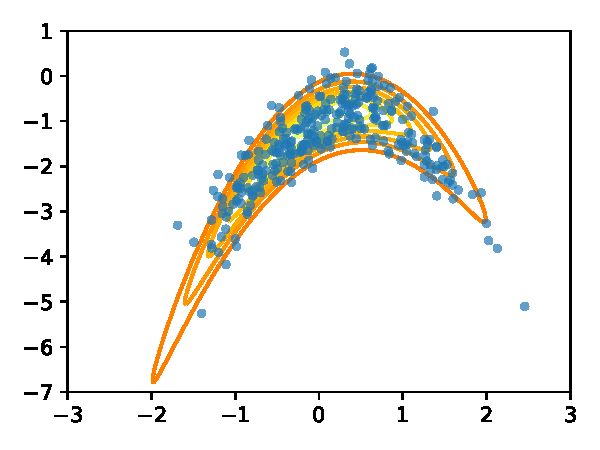
\includegraphics[width=0.335\textwidth]{syn_func_1.pdf} 
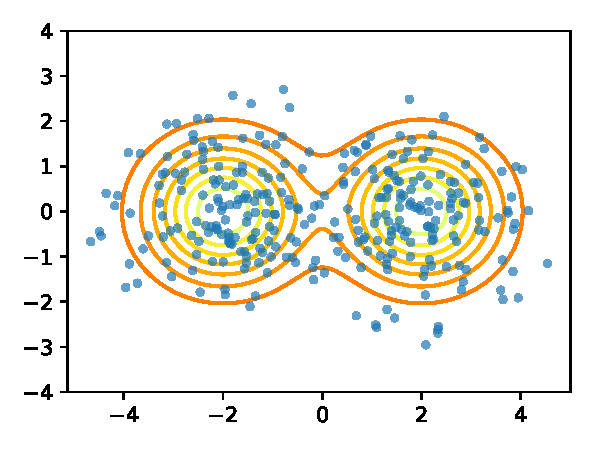
\includegraphics[width=0.335\textwidth]{syn_func_2.pdf} 
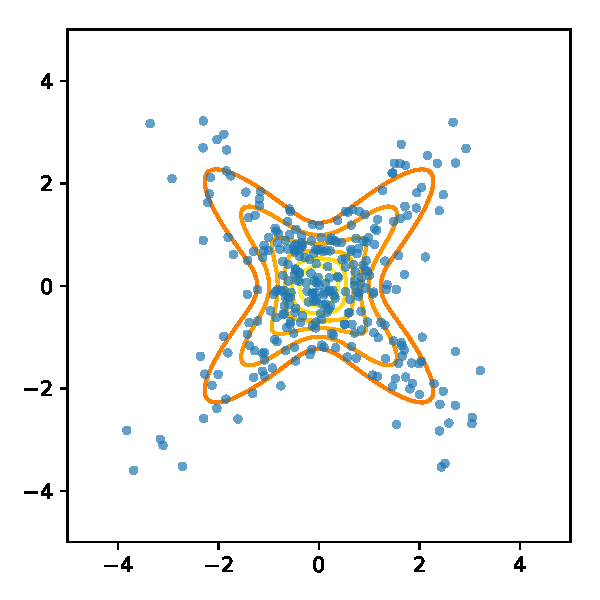
\includegraphics[width=0.24\textwidth]{syn_func_3.pdf} 
\caption{The contour plots of the synthetic distributions and the samples drawn from the variational distributions matching with the synthetic distributions using \us. }\label{fig:syn_dist}
\end{figure*}

The idea of using latent variables in the variational posterior starts with using mixtures \citep{BishopEtAl1998, GershmanEtAl2012, SalimansKnowles2013, GuoEtAl2016, MillerEtAl2017} and later extends with hierarchical models \citep{TranEtAl2015, RanganathEtAl2016, MaaloeEtAl2016}. To resolve the issue of computing the marginal PDF of variational posterior, \cite{AgakovBarber2004, RanganathEtAl2016, TranEtAl2015, MaaloeEtAl2016} exploit an auxiliary variable / distribution to derive a variational lower bound.

\section{Experiments}

We demonstrate the performance of \us as a variational posterior in several tasks. 
%We first shows the ability of \us for capturing complex distributions. In Section \ref{sec:exp_vae}, we demonstrate \us in amortized inference by using it to construct the encoder of a variational autoencoder \citep[VAE]{KingmaWelling2014}. In Section \ref{sec:exp_bnn}, we use \us to construct the variational posterior for Bayesian neural network (BNN) from a lower dimensional initial distribution.

%\subsection{Synthetic distributions}

\textbf{Synthetic distributions.} We first demonstrate the capability of \us in terms of capturing complex distributions. We use \us to match three synthetic distributions by minimizing the KL divergence between the variational distribution and the synthetic distribution $\KL{q(\xV)}{p(\xV)}$. We take the synthetic distribution used in \citep{YinZhou2018,TitsiasRuiz2019}. For all the synthetic distributions, we use a 2D normal distribution $\zV \sim \mathcal{N}(0,\I)$ as the initial distribution and use a DNN with two hidden layers with 50 hidden units and rectified linear (ReLU) unit as the transformation function. The auxiliary distribution uses a DNN with a mirrored architecture as the transformation function. We randomly initialized the weights of all the DNNs and initialized $\alpha=\sigma(-7)$ and $\beta=\sigma(-5)$, where $\sigma(a) = \log(1+\exp(a))$ is the soft-plus function. The number of samples used in learning is 1000. We optimize the lower bound using Adam \citep{KingmaBa2015} with the learning rate set to $0.001$ for the 100,000 iterations. 
%

%
The contour plots of the synthetic distributions and 300 samples drawn from the fitted variational distributions are shown in Fig.\,\ref{fig:syn_dist}. The samples from the fitted distributions match well with all the synthetic distribution. Note that, although the auxiliary distribution of \us encourages a one-to-one mapping between $\zV$ and $\xV$, it does not prevent \us from generating multi-modal distributions.

%\subsection{Variational autoencoder} \label{sec:exp_vae}

\textbf{Variational autoencoder.} Latent variable models such as the variational autoencoder (VAE) \citep{KingmaWelling2014} model the generation process from a latent representation $\xV$ to an observed data point $\yV$ as a conditional distribution $p(\yV|\xV)$. With a typically un-informative prior distribution $p(\xV)$, the goal is to learn the parameters of the conditional distribution $p(\yV|\xV)$, while estimating the posterior distribution $p(\xV|\yV)$. Such a model, especially a VAE, is a common choice for evaluating many variational inference methods, as learning a good generative model $p(\yV|\xV)$ requires a good mechanism for estimating variational posteriors $p(\xV|\yV)$. 

We compare with previous works by using \us to represent the variational posterior of a VAE. As a VAE uses amortized inference, the variational posterior $q(\xV|\yV)$ depends on the observed data representation $\yV$. When applying \us, we concatenate the data representation $\yV$ with the initial random variable $\zV$ and use a DNN as the transformation function that takes the concatenated representation as the input. The initial random variable $\zV$ follows a normal distribution of which the dimensionality is the same as $\xV$. The DNN has two hidden layers with ReLU non-linearity. The DNN in the auxiliary distribution has the mirrored architecture. We initialize $\alpha=\sigma(-5)$ and $\beta=\sigma(-3)$, of which the values are chosen according to a validation set.

We train VAE on two standard datasets: stochastically binarized MNIST \citep{SalakhutdinovMurray2008} and Fashion-MNIST \citep{XiaoEtAl2017}. Both datasets have 60,000 images of 28x28 resolution for training and 10,000 images for testing. We follow \citep{TitsiasRuiz2019} to binarize the Fashion-MNIST images by thresholding at 0.5. For the VAE, we model binary data by applying a Sigmoid transformation to the output of the DNN and use the outcome as the probability of a Bernoulli distribution. The dimensionality of $\xV$ is ten. The DNN in the VAE $p(\yV|\xV)$ has two hidden layers with 200 hidden units and ReLU non-linearity. The performance of a model is evaluated as the average marginal likelihood log-likelihood of the VAE on the set of test images. The marginal log-likelihood is estimated via importance sampling as in (\ref{eqn:importance_sampling}). This estimator has lower variance comparing to the importance sampling approach used in \citep{YinZhou2018, TitsiasRuiz2019}.
%
The results of \us are compared with previous methods in Tab.\,\ref{tab:vae}.

\begin{table}[t]
\centering
 \begin{tabular}{c c c} 
 \hline
 method & MNIST & Fashion-MNIST  \\ [0.5ex] 
 \hline\hline
 \us & \textbf{-91.24} & -116.89 \\
 meanfield & -98.29 & -126.73  \\ 
 \citep{YinZhou2018} & -97.77 & -121.53 \\
 \citep{TitsiasRuiz2019} & -94.09 & \textbf{-110.72}  \\ 
 \hline
\end{tabular}
\caption{Test log-likelihood of VAE on binarized MNIST and binarized Fashion-MNIST} \label{tab:vae}
\vspace{-5mm}
\end{table}

\begin{figure*}[h]
\centering
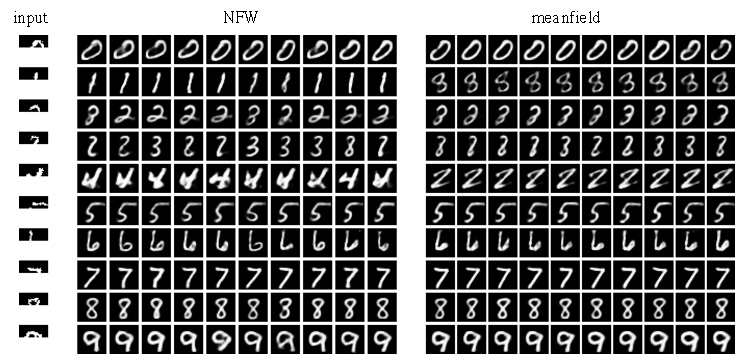
\includegraphics[width=0.95\textwidth]{mnist_imputation_wn.pdf} 
\caption{The image samples from the variational posteriors that are inferred from partially observed images. The partially observed images are shown in the 1st column. The samples from \us are shown in the middle column and the samples from mean field are shown in the 3rd column. } \label{fig:mnist_imp}
\end{figure*}

\textbf{Imputation with VAE.} After training a VAE, we demonstrate \us by inferring the posterior distribution of the VAE when the image is only partially observed. When only observing part of a handwritten digit, there are often multiple possibilities to complete the digit. A good posterior captures as many possibilities as possible. The requires the formulation of the posterior distribution to be very flexible. To set up such an experiment, we randomly select one image per digit and binarize the images by sampling from the Bernoulli distributions that take the normalized intensities as the probabilities of being one. We infer a variational posterior distribution for each image by only observing the top 12 rows of the binarized images, which are shown in the first column in Fig.\,\ref{fig:mnist_imp}. We compare \us and mean field on this task using the same VAE. For \us, we use a 10D normal distribution as the initial distribution and use a two hidden layer DNN with 300 hidden units as the transformation function. The optimization scheme is the same as for training the VAE. For each image, we randomly draw 10 samples from the inferred variational posterior and visualize in Fig.\,\ref{fig:mnist_imp}, where the middle column contains the samples from \us and the right column contains the samples from the mean field posterior. The samples from \us are more diverse, as \us provides a more expressive posterior representation comparing to the mean field posterior.

%\subsection{Bayesian neural network regression} \label{sec:exp_bnn}

\begin{table*}[h]
\centering
 \begin{tabular}{c c c c c} 
 \hline
 dataset & \us & meanfield  & PBP & Dropout \\ [0.5ex] 
 \hline\hline
 kin8nm & \textbf{1.19 (0.03)} & 1.16 (0.03) &  0.90 (0.01) & 0.95 (0.01)\\ 
 power & \textbf{-2.78 (0.04)} &  -2.79 (0.03) & -2.84 (0.01) & -2.80 (0.01)\\
 energy & \textbf{-1.32 (0.21)} & -1.59 (0.11)  & -2.04 (0.02) & -1.99 (0.02)\\
 concrete & -3.05 (0.19) & -3.07 (0.16) & -3.16 (0.02) & \textbf{-3.04 (0.02)}\\
 \hline
\end{tabular}
\vspace{1mm}
\caption{The average test log-likelihood of BNN on UCI regression benchmarks. The shown results are the average of 20 random partitions and the standard deviations are shown in parentheses.} \label{tab:bnn_regression}
\vspace{-5mm}
\end{table*}

\textbf{BNN regression.} A major challenge of using NF for BNN is the dimensionality of the variational distribution. With a non-invertible transformation, we can easily construct a correlated high dimensional variational posterior. We use \us to construct the variational posterior for BNN and evaluated on a few UCI regression benchmarks. We follow the common protocol of using 90\% for training and 10\% for testing. The experiments are repeated 20 times with different random partitions. For all the regression datasets and runs, we use the same settings. The BNN has one hidden layer with 50 units and ReLU non-linearity. The dimensionality of the initial distribution is 100, the transformation function is a DNN with two hidden layers (300-500 units) and ReLU non-linearity. We optimize with Adam using the learning rate of 0.01 for 1000k iterations and 0.001 for another 1000k iterations. The number of samples is 10. We initialize $\alpha=\sigma(-5)$ and $\beta=\sigma(-3)$. We compare our method with the meanfield variational posterior with the reparameterization trick. The results are shown in Tab.\,\ref{tab:bnn_regression}. The results of \us and meanfield use the same set of random partitions. The results of proba-bilistic backpropagation (PBP) \citep{hernandezAdams2015} and Dropout \citep{GalGhahramani2016} are directly taken from the papers.

\section{Conclusion}

We show that the PDF of the resulting distribution that is transformed with a non-invertible function can be derived analytically. To address the issue about computing all the real roots of the transformation equation, we derive a variational lower bound by introducing an auxiliary distribution. We demonstrate that the auxiliary distribution in \us produces a similar regularization effect as the log determinant in NF when the transformation is invertible. This provides some insights about the connection between the NF-based methods and the SIVI methods.

{
\bibliographystyle{plainnat}
\bibliography{nfw}
}

\newpage
\setcounter{page}{1}

\appendix
\onecolumn

    \begin{center}{\textbf{\LARGE Supplementary Material:}}
    \end{center}

    \begin{center}{\textbf{\Large Variational Inference with Non-invertible Flows}}
    \end{center}
    \vspace{0.3in}



\section{The analysis of the regularization term under 1D linear transformation}

Consider a 1D random variable $z$ following a normal distribution $q(z) = \gaussianDist{z}{0}{1}$ and apply a linear function $x=f(z)=wz$. According to the change of variable, the PDF of the random variable $x$ is
\begin{equation}
\log q(x) = \log \phi(\frac{x}{w})+ \log \left| \frac{\diff f^{-1}(x)}{\diff x} \right|^{-1} = \log \phi(\frac{x}{w}) - \log|w|,
\end{equation}
where $\phi(\cdot)$ is the PDF of the standard normal distribution. From the above equation, we denote the regularization term of NF to be $\gamma_{\text{NF}}(w) = \log|w|$.

With the same initial distribution $q(z)$ and the transformation function $f(z)$, we apply \us for VI by assuming $q(x|z) = \gaussianDist{x}{f(z)}{\alpha}$ and $\tilde{q}(z|x) = \gaussianDist{z}{\tilde{f}(x)}{\beta}$. Plugging them into (\ref{eqn:nfw_bound}), the regularization term becomes
\begin{equation}
\gamma_{\text{\us}} = \expectationDist{\log \frac{\tilde{q}(z | x)}{q(x|z)}}{q(x,z)} = \expectationDist{\log \frac{\gaussianDist{z}{\tilde{f}(x)}{\beta}}{\gaussianDist{x}{f(z)}{\alpha}}}{q(x,z)}.
\end{equation}

Assume the reverse transformation is also a linear function $\tilde{f}(x) = \tilde{w}x$ and plug it into the above equation. The regularization term of \us can be derived as 
\begin{align*}
\gamma_{\text{\us}} =& \expectationDist{\log \frac{\phi(\frac{\tilde{f}(f(z) + \alpha^{\frac{1}{2}} \epsilon) - z}{\beta^{\frac{1}{2}}})\beta^{-\frac{1}{2}}}{\phi(\frac{f(z) + \alpha^{\frac{1}{2}} \epsilon - f(z)}{\alpha^{\frac{1}{2}}}) \alpha^{-\frac{1}{2}}}}{q(z) q(\epsilon)} \\
=& \expectationDist{\log\phi(\frac{\tilde{f}(f(z) + \alpha^{\frac{1}{2}} \epsilon) - z}{\beta^{\frac{1}{2}}})}{q(z) q(\epsilon)} - \frac{1}{2}\log \beta - \expectationDist{\log \phi(\epsilon)}{q(\epsilon)} + \frac{1}{2}\log \alpha \\
=& -\frac{1}{2\beta}\expectationDist{\left(\tilde{w}(wz + \alpha^{\frac{1}{2}} \epsilon) - z\right)^2}{q(z) q(\epsilon)} - \frac{1}{2}\log \beta +\frac{1}{2} + \frac{1}{2}\log \alpha \\
=& -\frac{1}{2\beta}\left(1 - 2\tilde{w}w  + \tilde{w}^2w^2+\tilde{w}^2\alpha\right) - \frac{1}{2}\log \beta +\frac{1}{2} + \frac{1}{2}\log \alpha
\end{align*}

By taking $\frac{\diff \gamma_{\text{\us}}}{\diff \tilde{w}}=0$, the optimal value of $\tilde{w}$ can be derived as 
$$
\tilde{w}^* = \frac{w}{w^2+\alpha}.
$$

By plugging in the optimal $\tilde{w}$, we get the regularization term as a function of $w$,
$$
\gamma_{\text{\us}}(w)  = -\frac{1}{2\beta}\frac{\alpha}{w^2+\alpha} - \frac{1}{2}\log \beta +\frac{1}{2} + \frac{1}{2}\log \alpha.
$$

Fig.\,\ref{fig:regularization} in the main text shows the comparison of $\gamma_{\text{NF}}(w)$ and $\gamma_{\text{\us}}(w)$ with three different choices of $\alpha$ and $\beta$. These two regularization terms are both concave with the same minimum location. The smaller $\alpha$ and $\beta$ are, the steeper the regularization term is in \us. 

\section{Locally linear approximation}

Another way to understand to the connection between the regularization term in \us and in NF is to make a local linear approximation of the reverse transformation $\tilde{f}(\xV)$. In (\ref{eqn:regularization_term}), the transformed value $f(\zV)$ is corrupted with a small Gaussian noise $\xV = f(\zV) + \alpha^{\frac{1}{2}} \epsilon$. As the noise corruption will be small, we can do a Taylor expansion on $\tilde{f}$ around $f(\zV)$ and approximate it with a locally linear function,
$$
\tilde{f}(\xV) \approx \tilde{f}(\xV_0) +  \tilde{\J}_{\xV_0}^\top(\xV - \xV_0),
$$
where $\xV_0 = f(\zV)$ and $ \tilde{\J}_{\xV_0}$ is the Jacobian of $\tilde{f}$ at $\xV_0$. 

Plugging the above approximation into (\ref{eqn:nfw_bound}), we derive an approximated regularization term,
 \begin{align*}
\gamma_{\text{\us}} \approx& \expectationDist{\log \frac{\gaussianDist{\zV}{\tilde{f}(\xV_0) +  \tilde{\J}_{\xV_0}^\top(\xV - \xV_0)}{\beta}}{\gaussianDist{\xV}{f(\zV)}{\alpha}}}{q(\xV,\zV)} \\
=& \expectationDist{-\frac{1}{2\beta}\left( |\tilde{\zV} - \zV|^2 + \alpha \tr{\tilde{\J}_{\xV_0}^\top \tilde{\J}_{\xV_0}} \right)}{q(\zV)} - \frac{D_z}{2}\log (2\pi\beta) +\frac{D_x}{2} + \frac{D_x}{2}\log (2\pi\alpha)
\end{align*}
where $\tilde{\zV} = \tilde{f}( f(\zV) + \alpha^{\frac{1}{2}} \epsilon)$.
Compare the above term with the regularization term of NF in (\ref{eqn:mc_bound_nf}), which is
$$
\gamma_{NF} = -\expectationDist{\log \left| \frac{\diff f^{-1}(\xV)}{\diff \xV}\right|}{q(\zV)}.
$$
In the ideal situation, if the reverse transformation $\tilde{f}$ recovers the initial variable $\zV$ with sufficient accuracy, we can ignore the term $|\tilde{\zV} - \zV|^2$. Then, $\gamma_{\text{\us}}$ is dominated by the trace term.  In this case, if $f$ is invertible, $\tilde{f}$ will be close to $f^{-1}$. The term $-\frac{\alpha}{2\beta} \tr{\tilde{\J}_{\xV_0}^\top \tilde{\J}_{\xV_0}}$ encourages the Eigen values of the Jacobian of $f^{-1}$ to be smaller, which has a similar effect as $-\log \left| \frac{\diff f^{-1}(\xV)}{\diff \xV}\right|$ due to the connection between a determinant and a trace.

\end{document}
